\documentclass[11pt,a4paper]{article}

\usepackage[top=1.8cm,bottom=1.8cm,left=2cm,right=2cm]{geometry}
\usepackage[T1]{fontenc}
\usepackage[utf8]{inputenc}
\usepackage[english]{babel}
\usepackage{lmodern}
\usepackage{microtype}
\usepackage{graphicx}
\graphicspath{{figures/}}
\usepackage{booktabs}
\usepackage{amsmath}
\usepackage{float}
\usepackage{caption}
\usepackage{hyperref}
\usepackage{xurl}
\usepackage[round,authoryear]{natbib}

\hypersetup{colorlinks=true,linkcolor=black,citecolor=black,urlcolor=black}
\urlstyle{same}
\captionsetup{font=small,labelfont=bf,skip=5pt}
\setlength{\parindent}{0pt}
\setlength{\parskip}{3pt}
\setlength{\intextsep}{8pt plus 2pt minus 2pt}
\setlength{\textfloatsep}{10pt plus 2pt minus 2pt}
\emergencystretch=2em
\renewcommand{\refname}{References}

\begin{document}

\begin{center}
{\LARGE Competitive positioning of European semiconductor supply-chain firms in the AI era: a comparative analysis (2021--2025)}

\vspace{0.7cm}
{\large Salvatore Megna}

\vspace{0.25cm}
August 2026
\end{center}

\vspace{0.5cm}

\section{Introduction and objective of the analysis}

In recent years, the rapid adoption of artificial intelligence has increased demand for computing capacity and strengthened the role of advanced semiconductors in digital infrastructure. The development of increasingly complex processors, memories and architectures involves not only chip manufacturers but also the companies supplying the technologies required for fabrication, packaging and testing.

Several highly specialized European companies operate at different stages of this supply chain. ASML, ASM International, Besi, AIXTRON, VAT Group and Technoprobe supply technologies ranging from lithography and material deposition to advanced packaging, vacuum systems and semiconductor testing. Together, they cover several strategic stages of the semiconductor technology supply chain, forming a useful group for comparing financial performance over time.

The analysis covers 2021--2025 and examines company developments through revenue growth, research and development intensity, operating profitability, asset utilization and financial structure. The year 2020 is used as the initial reference for indexed revenue trajectories and R&D intensity. Comparisons consider both each company's development over time and the annual sample median as a common summary benchmark.

The study aims to describe changes in the financial and competitive positioning of the selected firms, identifying differences in growth, innovation, profitability and financial balance. The expansion of artificial intelligence applications provides the industrial context for this comparison; the analysis itself remains focused on financial performance observed in company financial statements.

\section{Sample, indicators and benchmarking framework}

\subsection{Companies included in the analysis}

The selection focuses on listed European companies supplying technologies for semiconductor production and testing, for which continuous and comparable financial information is available throughout the study period.

The sample includes six companies operating at strategic stages of the supply chain: ASML in lithography; ASM International and AIXTRON in deposition technologies; Besi in advanced packaging; VAT Group in vacuum systems; and Technoprobe in semiconductor testing. This composition makes it possible to examine firms exposed to distinct segments of the same European technology supply chain.

\begin{table}[H]
\centering
\caption{Companies included in the analysis}
\small
\begin{tabular}{lll}
\toprule
\textbf{Company} & \textbf{Country} & \textbf{Main technology segment} \\
\midrule
ASML & Netherlands & Lithography \\
ASM International & Netherlands & Deposition and wafer processing \\
Besi & Netherlands & Advanced packaging \\
AIXTRON & Germany & Deposition technologies \\
VAT Group & Switzerland & High-vacuum technologies \\
Technoprobe & Italy & Semiconductor testing \\
\bottomrule
\end{tabular}
\end{table}

\subsection{Data, indicators and comparison criteria}

The data were obtained from the companies' consolidated financial statements and official annual reports. The principal items used are revenue, operating income, research and development expenditure, total assets, current assets and liabilities, and shareholders' equity. The specific sources associated with the raw data were recorded in the working dataset.

Five main indicators were constructed from this information: annual revenue growth, return on sales (ROS), R&D intensity, asset turnover and equity autonomy. The current ratio was also used to assess liquidity, but was not included in the subsequent principal component analysis.

Company expansion is also represented using indexed revenue, with the 2020 value set to 100. This transformation makes company trajectories comparable regardless of initial size or financial-reporting currency. R&D intensity is the ratio of research and development expenditure to revenue; ROS is operating income divided by revenue; asset turnover measures the ability to generate revenue from the asset base; equity autonomy is the share of total assets financed by equity; and the current ratio compares current assets with current liabilities.

For each indicator, the benchmark is the annual median of the six companies. In the charts, this common reference makes it possible to assess each firm's relative position alongside its time trajectory.

\subsection{Descriptive profile of the sample}

The dataset used for benchmarking and the subsequent multivariate analysis contains 30 company--year observations, representing six firms during 2021--2025, with no missing values in the indicators considered. The year 2020 is not an additional observation in the analytical dataset: it is used only as the base year for indexed revenue and as an initial reference in the R&D intensity chart.

\begin{table}[H]
\centering
\caption{Descriptive statistics for financial indicators}
\small
\begin{tabular}{lrrrrrr}
\toprule
\textbf{Indicator} & \textbf{N} & \textbf{Mean} & \textbf{Median} & \textbf{Std. dev.} & \textbf{Min} & \textbf{Max} \\
\midrule
Revenue growth (\%) & 30 & 15,8 & 13,9 & 22,6 & -25,4 & 72,8 \\
R\&D intensity (\%) & 30 & 10,3 & 10,9 & 3,0 & 4,4 & 14,6 \\
ROS (\%) & 30 & 29,1 & 28,8 & 7,3 & 12,4 & 42,4 \\
Asset turnover & 30 & 0,65 & 0,63 & 0,13 & 0,44 & 0,98 \\
Equity autonomy (\%) & 30 & 64,7 & 68,7 & 18,6 & 29,1 & 88,0 \\
Current ratio & 30 & 3,72 & 3,07 & 2,12 & 1,24 & 8,06 \\
\bottomrule
\end{tabular}
\end{table}

The descriptive statistics show considerable variation across observations, particularly for revenue growth, financial structure and liquidity. The outlier check flags two unusually high observations: Besi's revenue growth in 2021 and VAT Group's asset turnover in 2022. Both were retained because they are consistent with the companies' financial statements. Marked differences among observations further support using the annual median rather than the mean as a benchmarking reference, because it is less affected by extreme values.

\section{Benchmarking evidence}

The collected information is now used to compare changes in the firms' principal financial dimensions. Benchmarking considers each company's trajectory together with the annual sample median, shown by the black dashed line in the charts. The comparison covers growth and innovation, profitability and asset-use efficiency, and financial strength and liquidity.

\subsection{Revenue expansion and innovation investment}

Revenue growth is represented by an index with 2020 = 100, while innovation investment is measured by the share of revenue devoted to research and development. The two measures allow comparisons of cumulative expansion and R&D expenditure relative to turnover, respectively.

\begin{figure}[H]
\centering
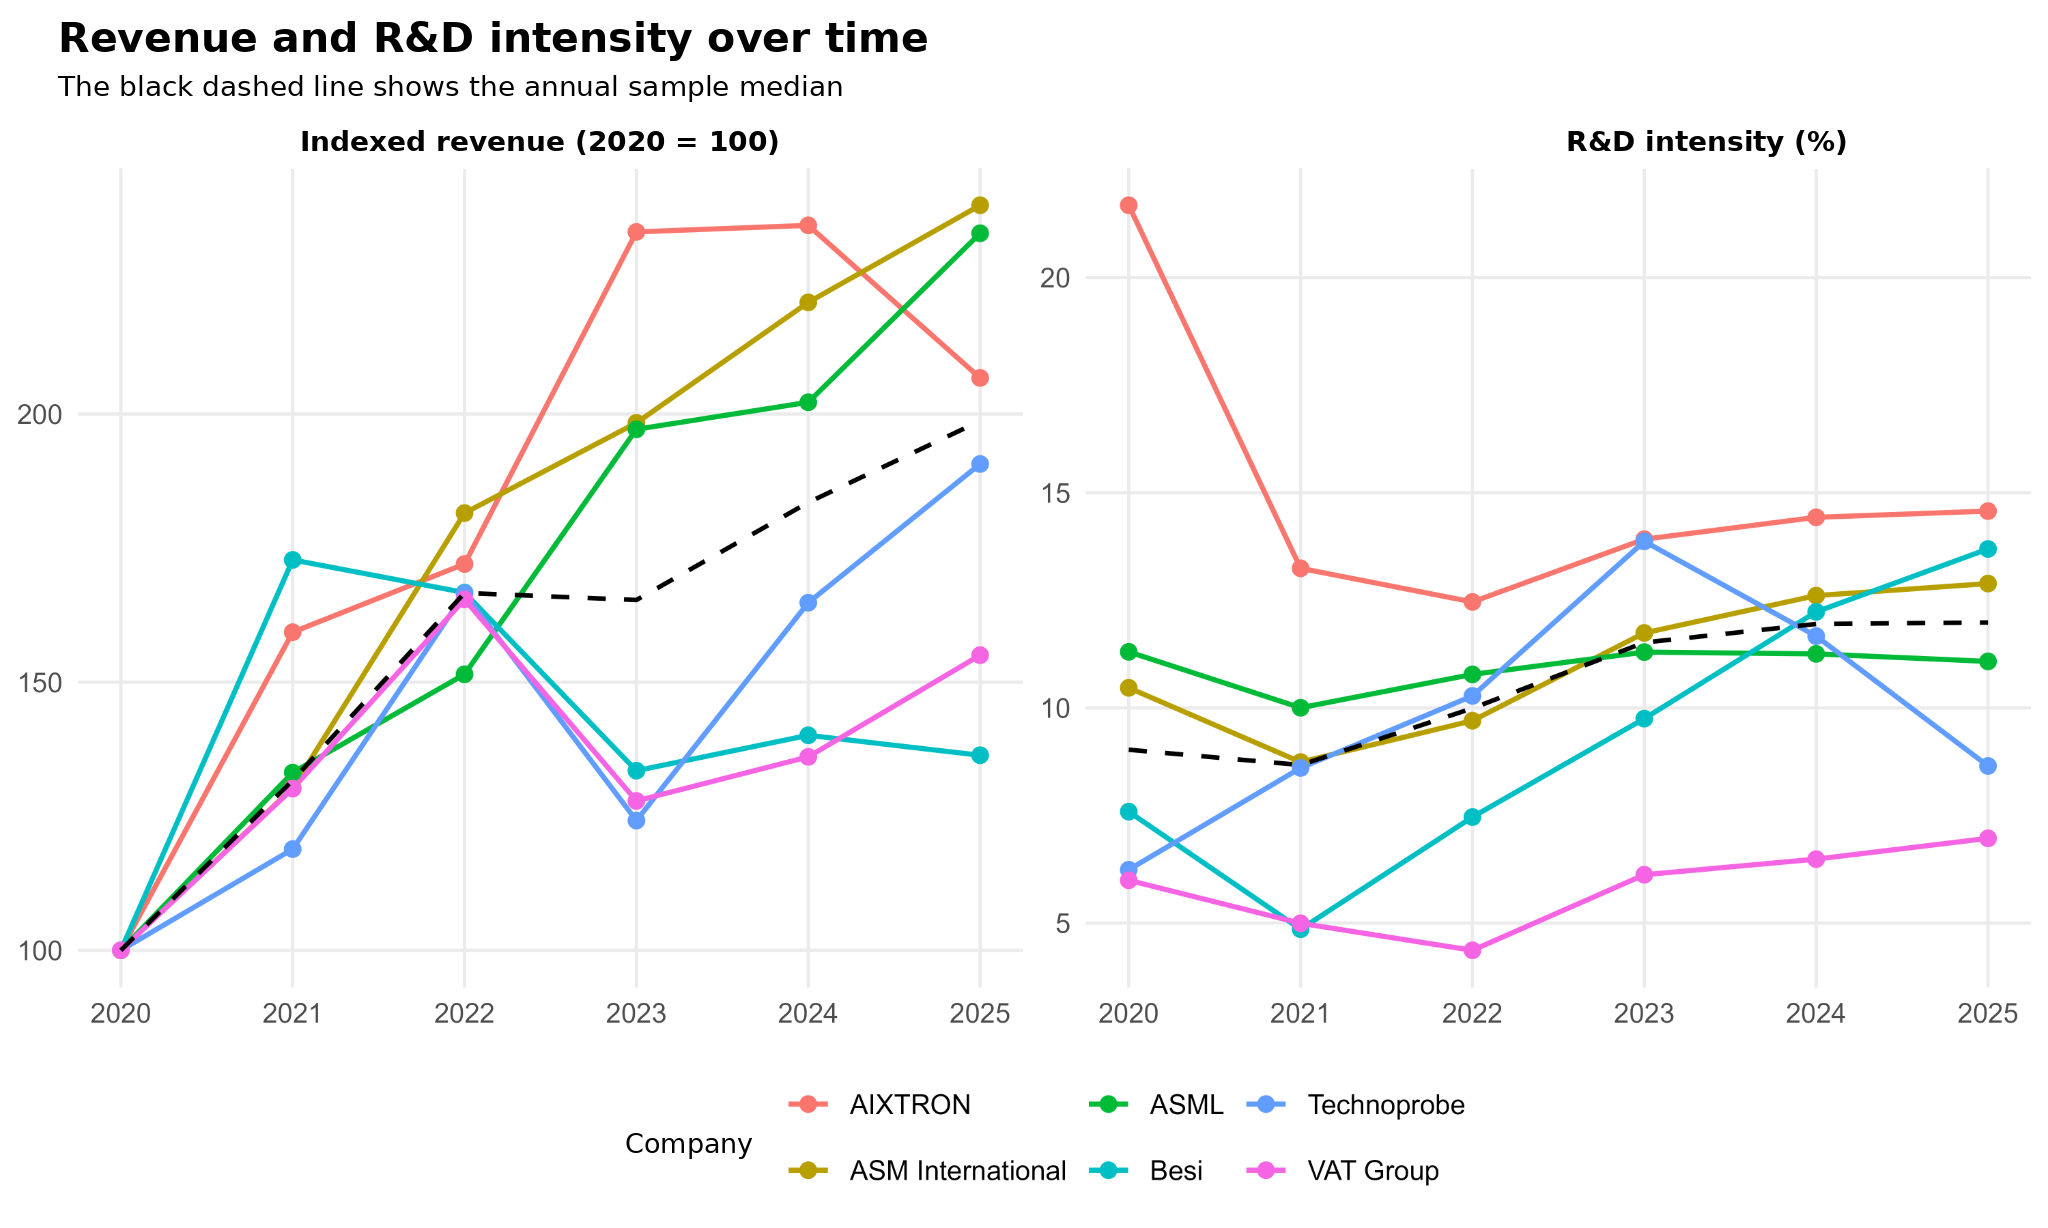
\includegraphics[width=0.94\textwidth]{01_crescita_innovazione_en.png}
\caption{Revenue and R\&D intensity over time}
\label{fig:crescita_innovazione}
\end{figure}

Figure~\ref{fig:crescita_innovazione} shows strong overall revenue expansion, but with different trajectories. Median indexed revenue rises from 100 in 2020 to approximately 167 in 2022, remains broadly stable in 2023, and then increases to about 199 in 2025. ASM International and ASML have the steadiest cumulative growth, reaching approximately 239 and 234, respectively, by the end of the period. AIXTRON accelerates sharply through 2023 before declining in 2025, while Besi and VAT Group show more modest growth overall. Technoprobe follows a more uneven path, contracting in 2023 and subsequently recovering.

The slowdown in 2023 occurred during a broader semiconductor-cycle correction. After record manufacturing investment in 2022, weaker chip demand and high inventory levels in the consumer and mobile segments caused a decline in spending on new facilities \citep{semi2023}. The same dynamics appear in Technoprobe's results: the company attributed its 2023 revenue decline to contraction in its reference market and high customer inventory levels \citep{technoprobe2023h1}.

The subsequent recovery was not uniform across the supply chain. ASM International, for example, is directly exposed to deposition technologies used in the most advanced nodes: in 2024 it reported strong demand linked to gate-all-around (GAA) architectures and high-bandwidth memory (HBM), identifying artificial intelligence as an important market driver \citep{asm2024q3}. Besi operates in advanced packaging, where rising demand for 2.5D solutions and data-center applications coexists with weakness in established markets such as mobile, automotive and industrial equipment \citep{besi2026}. Different exposures to the technology segments driving the recovery help explain why revenue rebounded with differing timing and intensity across firms.

R&D intensity also trends upward overall. The sample median increases from approximately 9\% in 2020 to about 12\% in 2025. AIXTRON remains above the benchmark for most of the period, while ASM International and Besi gradually increase their R&D intensity. Technoprobe reaches its highest value in 2023 before lowering R&D expenditure as a share of revenue in subsequent years.

AIXTRON's profile illustrates that high innovation intensity does not necessarily translate into steady revenue growth. The company focuses mainly on compound semiconductors and serves power-electronics and optoelectronics markets, among others. In 2025 demand for GaN and SiC power applications remained weak, while optoelectronics benefited from rising demand for lasers and photonic solutions for high-speed data transmission \citep{aixtron2026}. The final-year revenue decline can therefore also be understood in light of differing demand trends across its end markets. Overall, the increase in median R&D intensity suggests that the cyclical slowdown did not lead to a generalized reduction in innovation investment.

\subsection{Profitability and asset utilization}

To assess whether revenue expansion was accompanied by a similar improvement in operating performance, ROS and asset turnover are examined. ROS measures the share of revenue converted into operating income; asset turnover describes the company's ability to generate revenue from its asset base.

\begin{figure}[H]
\centering
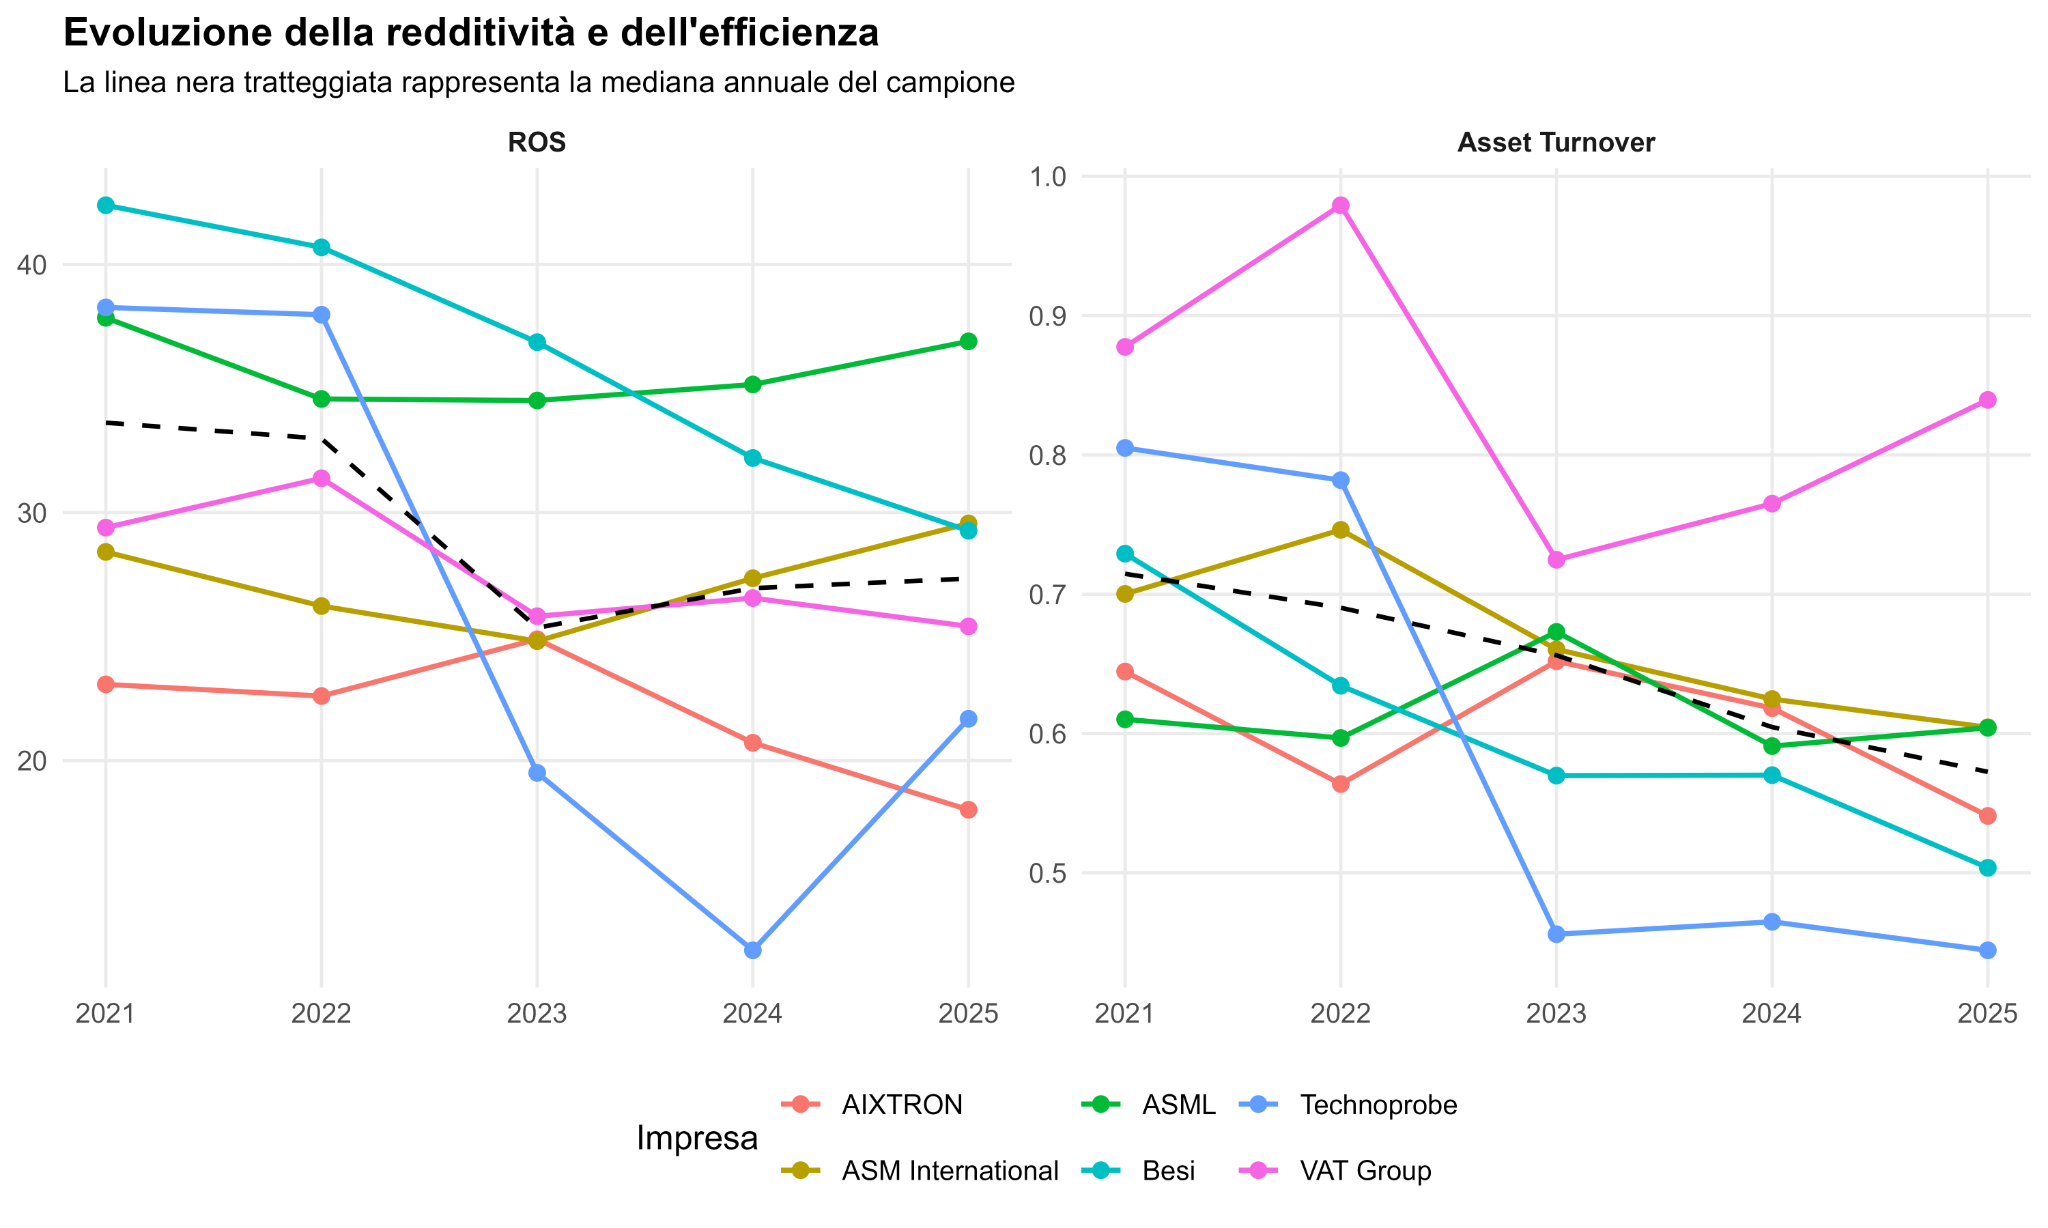
\includegraphics[width=0.94\textwidth]{02_redditivita_efficienza.png}
\caption{Evoluzione della redditività e dell'efficienza}
\label{fig:redditivita_efficienza}
\end{figure}

La Figura \ref{fig:redditivita_efficienza} mostra che la crescita osservata nei ricavi non si traduce in un miglioramento uniforme della redditività. Il ROS mediano si mantiene intorno al 33\% nel 2021--2022, scende a circa il 25\% nel 2023 e recupera solo parzialmente negli anni successivi, raggiungendo circa il 27\% nel 2025. ASML mantiene per tutto il periodo una redditività operativa superiore al benchmark e relativamente stabile. Besi parte da livelli ancora più elevati, ma mostra una progressiva riduzione del margine, mentre Technoprobe registra la variazione più marcata, passando da valori prossimi al 38\% nel 2021--2022 a circa il 12\% nel 2024, prima di recuperare nell'ultimo anno.

L'Asset Turnover presenta una riduzione più generalizzata: la mediana passa da circa 0,71 nel 2021 a 0,57 nel 2025. VAT Group mantiene i valori più elevati per quasi tutto il periodo, mentre Technoprobe mostra una forte riduzione a partire dal 2023. Il calo dell'indicatore segnala che, nel complesso, la crescita della base patrimoniale è stata più rapida della capacità di generare ricavi attraverso gli asset disponibili. Tale andamento non implica necessariamente un peggioramento dell'efficienza in senso assoluto, poiché può riflettere anche investimenti e ampliamenti della capacità destinati a sostenere la crescita futura.

Il caso di Technoprobe consente di leggere più chiaramente il legame tra ciclo di mercato, marginalità e utilizzo degli asset. Nel 2023 la riduzione della domanda e gli elevati livelli di inventario detenuti dai clienti hanno determinato una forte contrazione delle vendite. La minore attività produttiva ha ridotto l'assorbimento dei costi fissi, contribuendo alla compressione dei margini; contemporaneamente, la società ha scelto di mantenere la struttura produttiva e le risorse impiegate in previsione di una successiva ripresa dei volumi \citep{technoprobe2023h1}.

Nello stesso periodo Technoprobe ha continuato a sostenere gli investimenti produttivi e tecnologici e, nell'agosto 2023, ha acquisito Harbor Electronics, ampliando il proprio perimetro industriale nel settore dei circuiti stampati avanzati utilizzati nelle probe card \citep{technoprobe2024}. La contemporanea diminuzione del ROS e dell'Asset Turnover appare quindi coerente con una fase in cui i ricavi si sono ridotti mentre la capacità produttiva e la base di asset sono state in larga misura preservate e successivamente rafforzate. Il recupero dei ricavi osservato dal 2024 non determina infatti un immediato ritorno ai livelli di redditività e rotazione degli asset precedenti alla correzione.

Nel complesso, il confronto evidenzia una distinzione tra crescita dimensionale e performance operativa: le imprese che registrano la maggiore espansione dei ricavi non presentano necessariamente il miglioramento più marcato dei margini o della rotazione degli asset. Le differenti traiettorie riflettono quindi non soltanto l'andamento generale del mercato, ma anche il momento con cui i diversi segmenti della filiera attraversano le fasi di investimento, rallentamento e successivo recupero.

\subsection{Solidità patrimoniale e liquidità}

La struttura finanziaria viene analizzata attraverso l'autonomia finanziaria e il Current Ratio. Il primo indicatore misura l'incidenza del patrimonio netto sul totale dell'attivo, mentre il secondo consente di valutare l'equilibrio finanziario di breve periodo confrontando attività e passività correnti.

\begin{figure}[H]
\centering
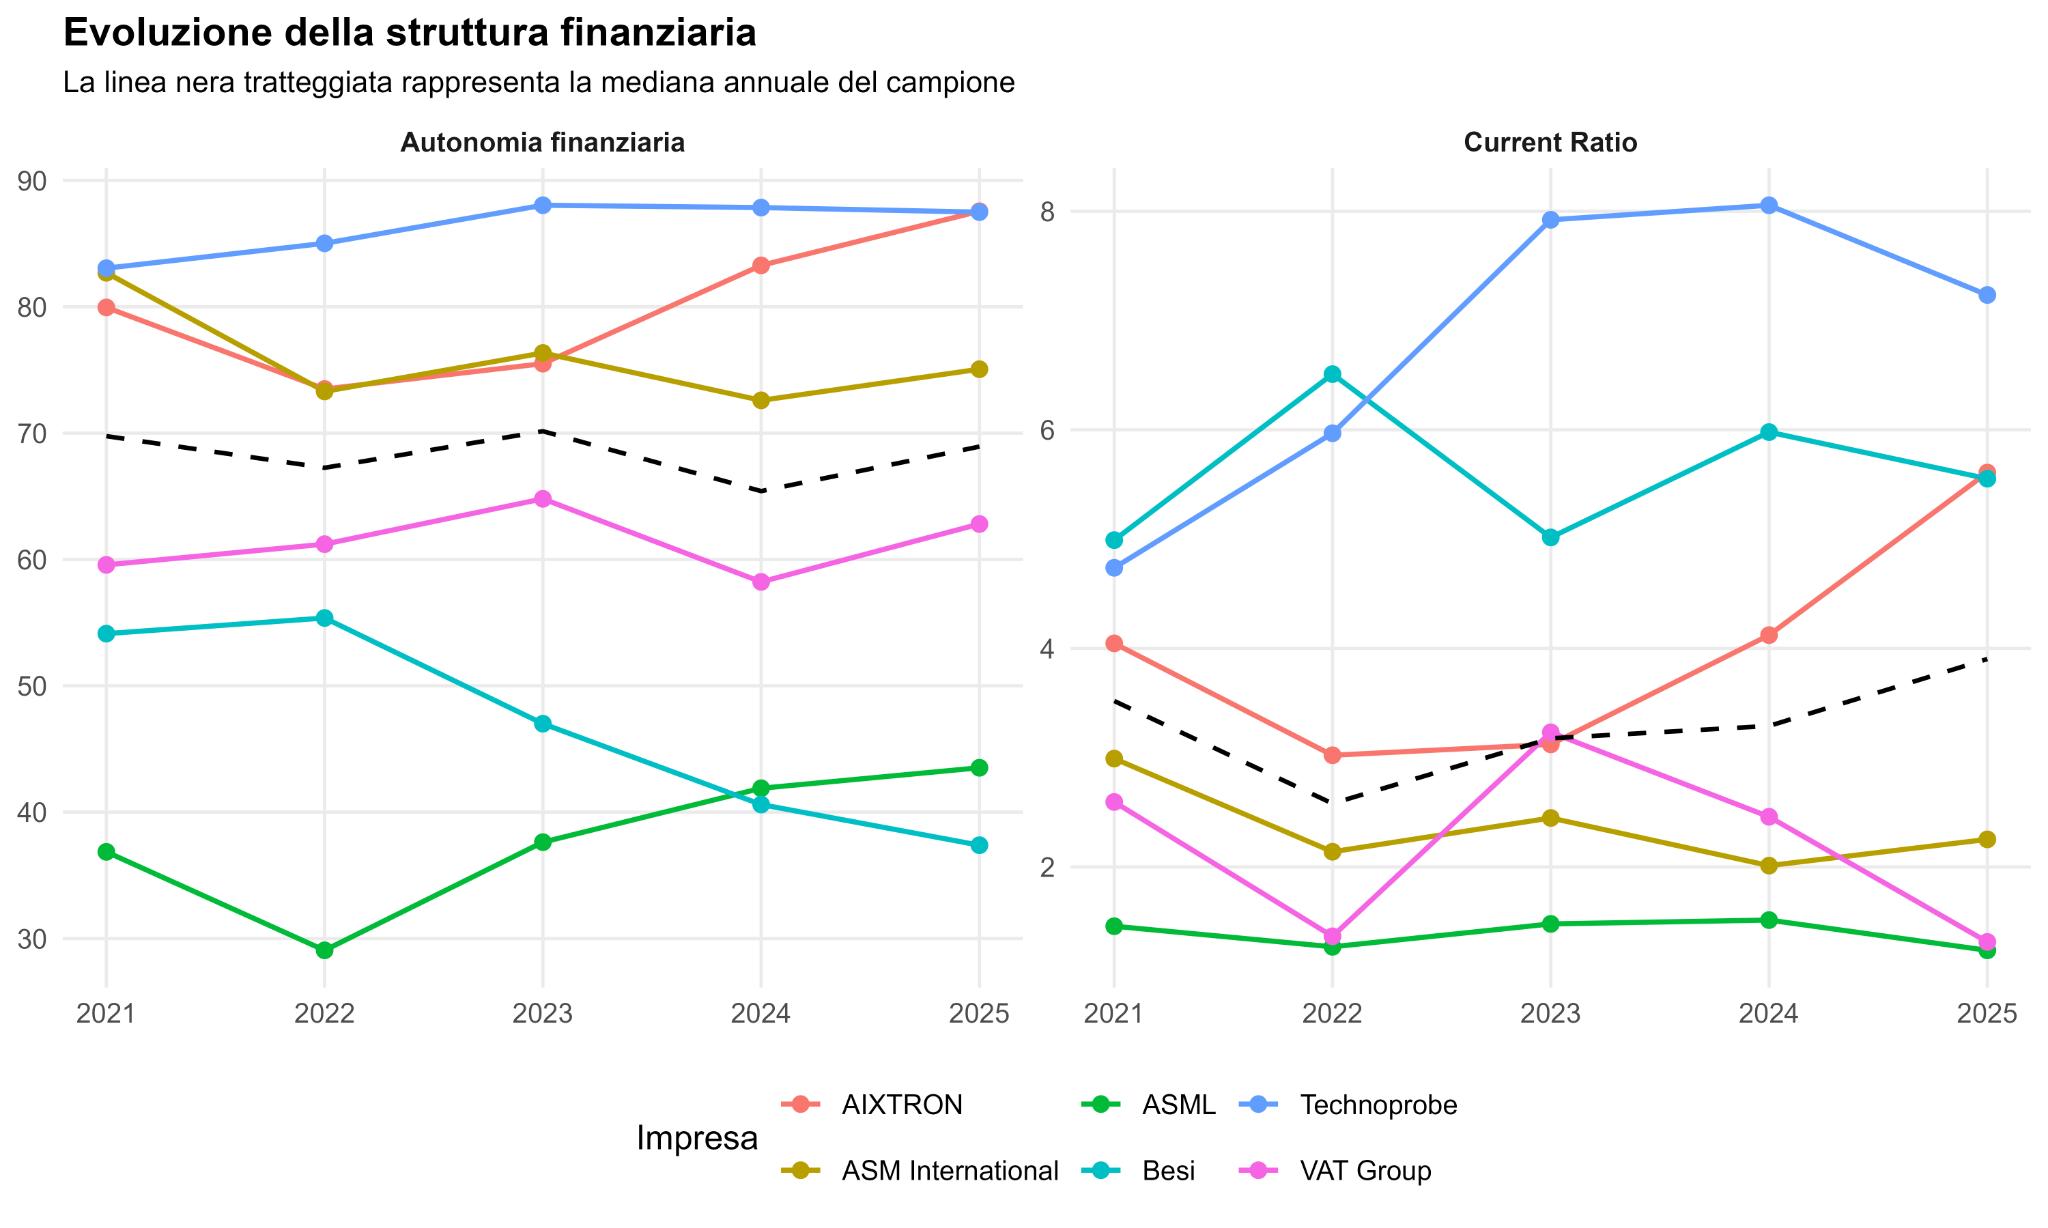
\includegraphics[width=0.94\textwidth]{03_struttura_finanziaria.png}
\caption{Evoluzione della struttura finanziaria}
\label{fig:struttura_finanziaria}
\end{figure}

La Figura \ref{fig:struttura_finanziaria} evidenzia profili finanziari nettamente differenziati. La mediana dell'autonomia finanziaria rimane complessivamente stabile, oscillando nel periodo tra circa il 65\% e il 70\%. Technoprobe presenta valori superiori all'80\% per l'intero periodo, mentre AIXTRON rafforza progressivamente la propria autonomia fino a raggiungere circa l'88\% nel 2025. Anche ASM International si mantiene stabilmente sopra il benchmark. ASML e Besi mostrano invece una minore incidenza del patrimonio netto sul totale dell'attivo, pur seguendo traiettorie differenti.

Le differenze risultano altrettanto evidenti nella liquidità. Il Current Ratio mediano scende da circa 3,5 nel 2021 a 2,6 nel 2022, per poi risalire progressivamente fino a circa 3,9 nel 2025. Technoprobe mantiene i valori più elevati nella parte finale del periodo, mentre Besi presenta anch'essa una liquidità ampiamente superiore al benchmark. ASML si colloca invece stabilmente su livelli inferiori alla mediana. In tutte le osservazioni il Current Ratio rimane comunque superiore a uno, indicando che le attività correnti risultano superiori alle passività correnti.

Il confronto mostra quindi che non emerge un unico profilo finanziario associato alle imprese con maggiore crescita o redditività. ASML, ad esempio, mantiene una redditività operativa tra le più elevate del campione pur presentando livelli di autonomia finanziaria e liquidità inferiori alla mediana. Technoprobe mostra invece una struttura patrimoniale particolarmente solida e un Current Ratio elevato, a fronte di una redditività che si riduce sensibilmente nel 2023--2024. Le diverse dimensioni della performance non coincidono pertanto in una graduatoria univoca, rendendo utile una successiva lettura congiunta attraverso l'Analisi in Componenti Principali.

\section{Profili competitivi e sintesi multidimensionale}

\subsection{Impostazione della PCA e capacità di sintesi}

Il benchmarking ha evidenziato come crescita, innovazione, redditività ed equilibrio finanziario non si muovano necessariamente nella stessa direzione. Per osservare congiuntamente queste dimensioni viene applicata un'Analisi in Componenti Principali (PCA), che consente di sintetizzare l'informazione contenuta negli indicatori originari in un numero più ridotto di componenti.

L'analisi è condotta sulle 30 osservazioni impresa--anno del periodo 2021--2025 e considera cinque variabili: crescita annuale dei ricavi, ROS, intensità di ricerca e sviluppo, Asset Turnover e autonomia finanziaria. Prima dell'applicazione della PCA, gli indicatori sono stati standardizzati, così da eliminare l'influenza delle differenti unità di misura e rendere confrontabile il loro contributo alla costruzione delle componenti.

\begin{table}[H]
\centering
\caption{Autovalori e varianza spiegata dalle componenti principali}
\small
\begin{tabular}{lrrr}
\toprule
\textbf{Componente} & \textbf{Autovalore} & \textbf{Varianza (\%)} & \textbf{Cumulata (\%)} \\
\midrule
PC1 & 2,309 & 46,2 & 46,2 \\
PC2 & 1,324 & 26,5 & 72,6 \\
PC3 & 0,784 & 15,7 & 88,3 \\
PC4 & 0,312 & 6,2 & 94,6 \\
PC5 & 0,271 & 5,4 & 100,0 \\
\bottomrule
\end{tabular}
\end{table}

Le prime due componenti presentano un autovalore superiore a uno e spiegano congiuntamente il 72,6\% della variabilità complessiva. La rappresentazione nel piano formato da PC1 e PC2 conserva quindi una quota ampia dell'informazione contenuta nei cinque indicatori e viene utilizzata per la lettura sintetica dei profili aziendali.

\subsection{Interpretazione delle componenti}

Per attribuire un significato economico alle due dimensioni trattenute, si osservano le associazioni tra gli indicatori originari e le componenti principali.

\begin{table}[H]
\centering
\caption{Associazione delle variabili originarie con PC1 e PC2}
\small
\begin{tabular}{lrr}
\toprule
\textbf{Variabile} & \textbf{PC1} & \textbf{PC2} \\
\midrule
Crescita ricavi ($\Delta$RIC) & -0,471 & 0,481 \\
ROS & -0,765 & -0,472 \\
Intensità R\&S & 0,809 & -0,227 \\
Asset Turnover (AT) & -0,778 & 0,438 \\
Autonomia finanziaria (AF) & 0,492 & 0,792 \\
\bottomrule
\end{tabular}
\end{table}

La prima componente, che spiega il 46,2\% della varianza, contrappone soprattutto l'intensità di ricerca e sviluppo e, in misura minore, l'autonomia finanziaria, alla redditività operativa e alla capacità di generare ricavi attraverso gli asset. Valori positivi di PC1 risultano quindi associati a una maggiore intensità di R\&S, mentre ROS e Asset Turnover presentano associazioni negative elevate.

La seconda componente spiega il 26,5\% della varianza ed è associata soprattutto all'autonomia finanziaria, alla quale si affiancano la crescita dei ricavi e l'Asset Turnover; sul lato opposto si colloca principalmente il ROS. PC2 può quindi essere letta soprattutto come una dimensione di solidità patrimoniale e dinamica di crescita. Il segno delle componenti è convenzionale: l'interpretazione riguarda le opposizioni tra variabili e non una scala automatica tra posizioni migliori e peggiori.

\subsection{Posizionamento e traiettorie delle imprese}

Il piano fattoriale consente di leggere contemporaneamente la posizione delle imprese e la loro evoluzione nel tempo. Le traiettorie vengono interpretate collegando gli spostamenti nel piano ai risultati emersi nel benchmarking, senza attribuire alle componenti un significato di graduatoria.

\begin{figure}[H]
\centering
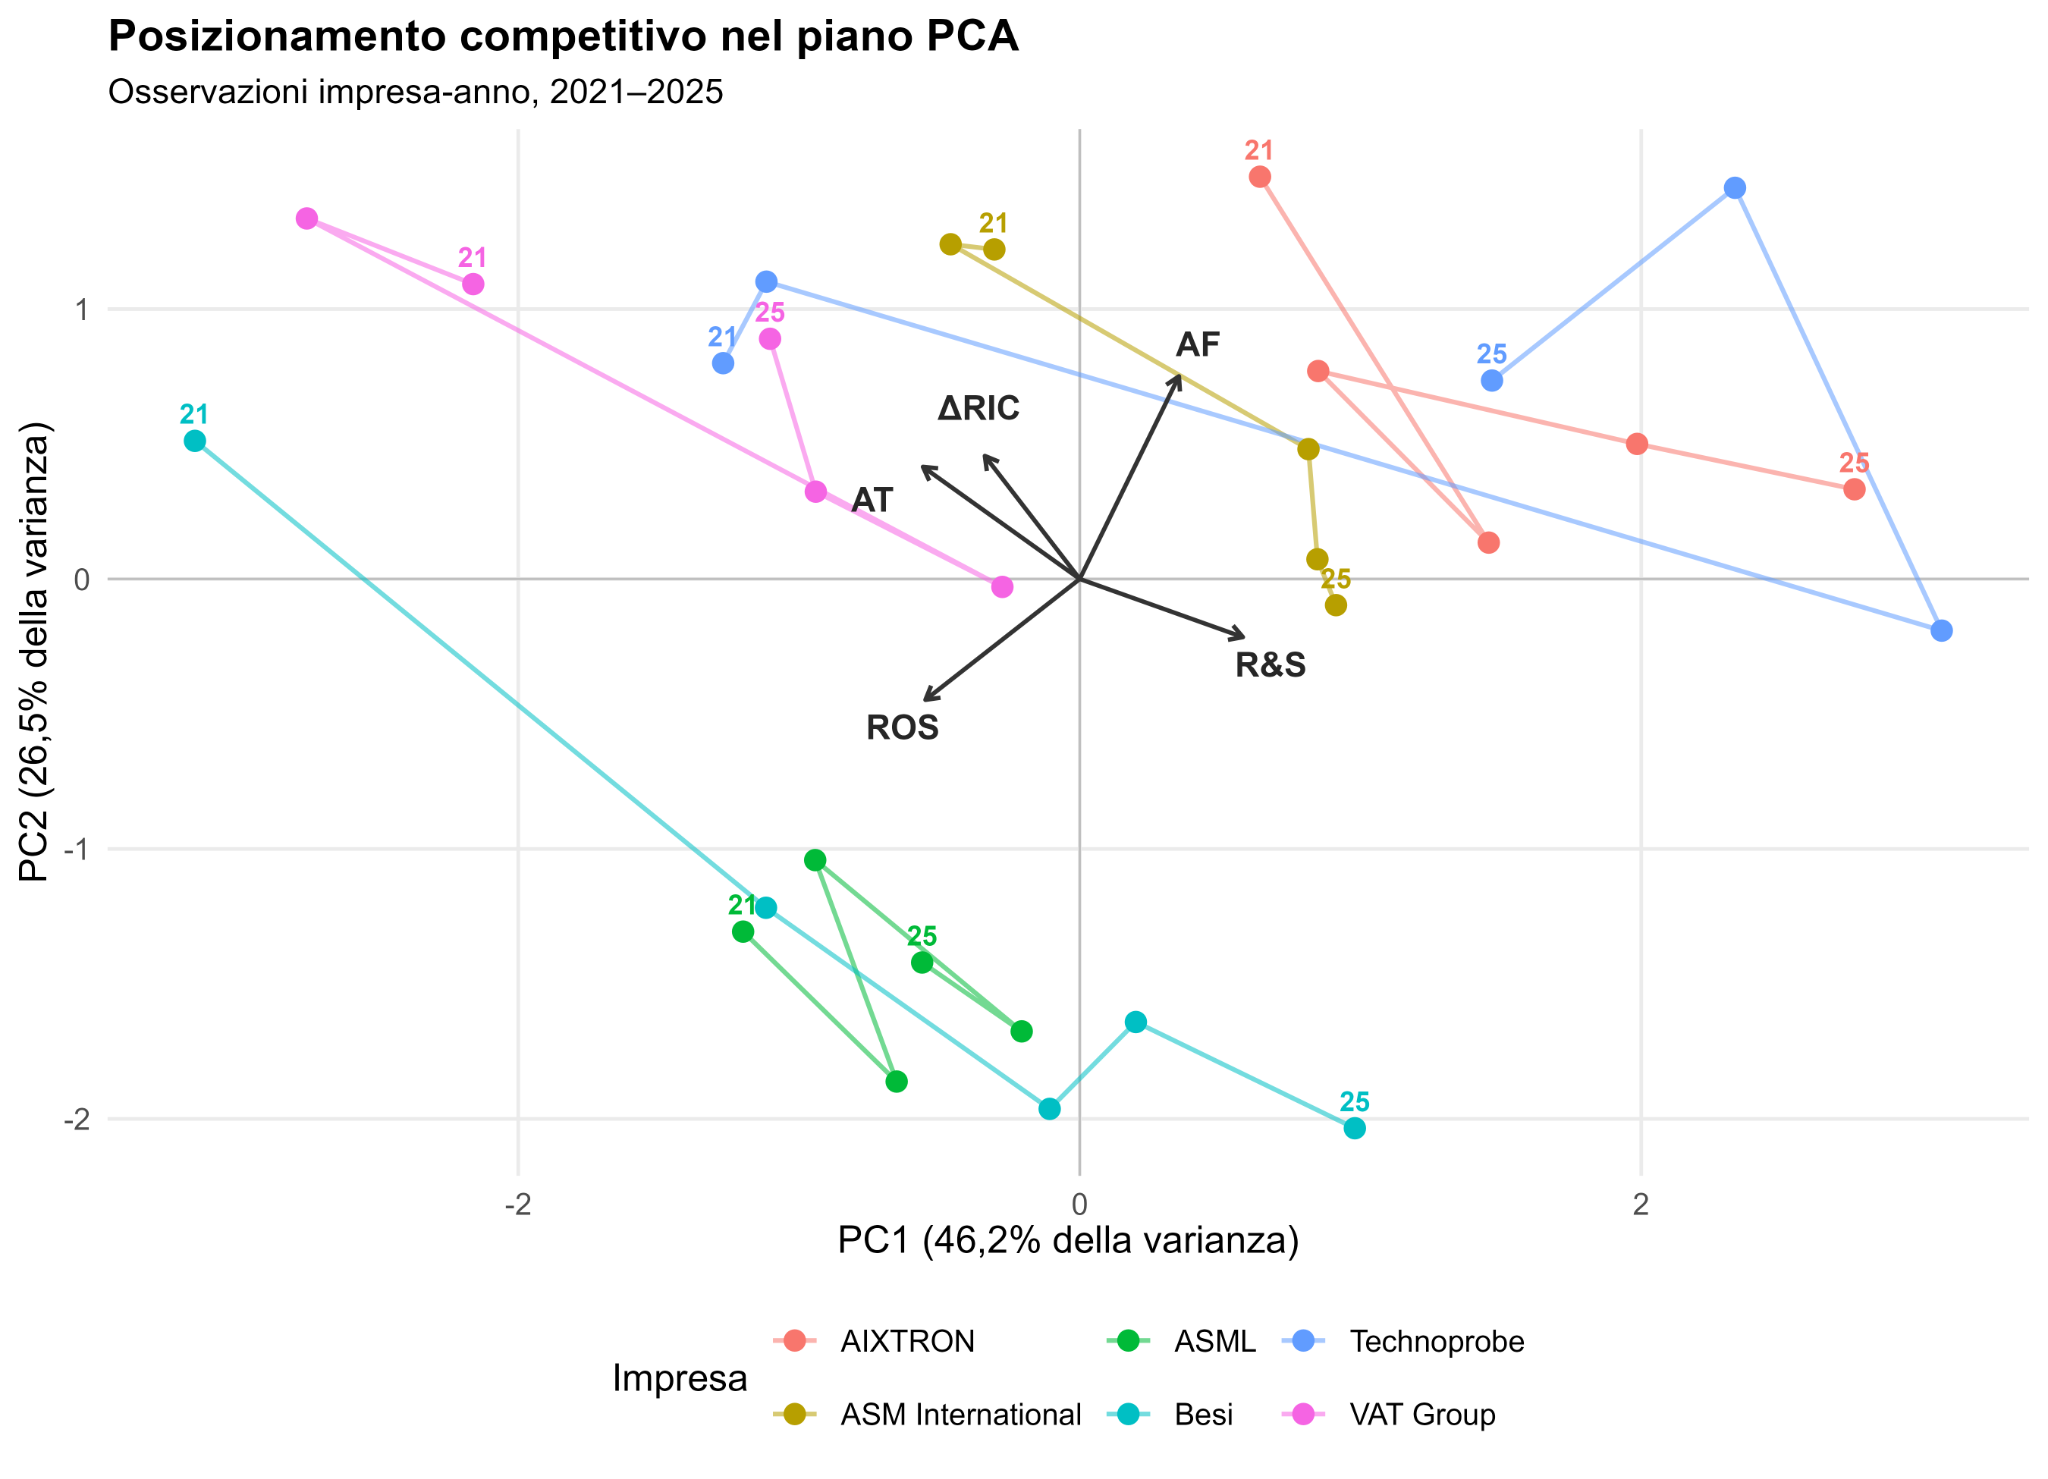
\includegraphics[width=0.92\textwidth]{04_pca_mappa_competitiva.png}
\caption{Posizionamento competitivo delle imprese nel piano PCA}
\label{fig:pca}
\end{figure}

La Figura \ref{fig:pca} mostra come le differenze osservate nel benchmarking si riflettano nel posizionamento congiunto delle imprese. L'origine del piano rappresenta il profilo medio delle osservazioni standardizzate dell'intero campione e non coincide con il benchmark mediano annuale utilizzato nei grafici precedenti.

\paragraph{AIXTRON e ASML.}
AIXTRON si colloca per l'intero periodo nel lato positivo della prima componente e si sposta ulteriormente verso destra nel 2025. Tale posizione è coerente con l'elevata intensità di ricerca e sviluppo e con la forte autonomia finanziaria, alle quali si accompagnano negli anni più recenti livelli più contenuti di redditività e rotazione degli asset. ASML presenta un profilo quasi speculare e rimane stabilmente nel quadrante inferiore sinistro: il suo posizionamento è associato soprattutto al ROS persistentemente elevato, mentre la minore autonomia finanziaria contribuisce ai valori negativi della seconda componente. Il confronto mette quindi in evidenza due configurazioni competitive differenti, una maggiormente caratterizzata dall'intensità innovativa e dalla solidità patrimoniale e l'altra dalla redditività operativa.

\paragraph{Besi.}
Besi mostra uno degli spostamenti più ampi nel piano fattoriale. Tra il 2021 e il 2025 l'impresa si muove dal quadrante superiore sinistro verso quello inferiore destro, passando da valori fortemente negativi a positivi su PC1 e, contemporaneamente, da valori positivi a fortemente negativi su PC2. Lo spostamento lungo PC1 è coerente con il progressivo aumento dell'intensità di R\&S e con la riduzione del ROS e dell'Asset Turnover; il movimento verso valori più bassi di PC2 riflette soprattutto il rallentamento della crescita e la diminuzione dell'autonomia finanziaria. La traiettoria descrive quindi una trasformazione del profilo dell'impresa, più che un semplice miglioramento o peggioramento complessivo.

\paragraph{Technoprobe.}
Technoprobe presenta una traiettoria altrettanto dinamica. Nel 2021--2022 si colloca nella parte superiore sinistra del piano, coerentemente con livelli elevati di ROS e Asset Turnover e con una forte autonomia finanziaria. Nel 2023 il profilo cambia nettamente: la crescita dei ricavi diventa negativa, il ROS scende da circa il 38\% al 19,5\% e l'Asset Turnover passa da 0,78 a circa 0,46, mentre l'intensità di R\&S raggiunge il valore massimo del periodo. Nel 2024 la redditività si riduce ulteriormente; nel 2025 la traiettoria torna invece parzialmente verso il centro, con un recupero del ROS e una struttura patrimoniale ancora molto solida. Il percorso evidenzia quindi una fase di forte discontinuità seguita da segnali di riequilibrio nell'ultimo anno.

Nel complesso, la PCA conferma che le imprese non possono essere ordinate secondo una graduatoria univoca. Il posizionamento dipende dalla combinazione tra crescita, innovazione, redditività, utilizzo degli asset e solidità finanziaria: società collocate in aree differenti del piano possono quindi presentare punti di forza su dimensioni diverse.

\section{Conclusioni}

Nel periodo 2021--2025 il campione mostra una forte espansione complessiva, interrotta dalla correzione ciclica del 2023 e seguita da una ripresa selettiva. La crescita dei ricavi si accompagna a un'intensità di ricerca e sviluppo mediamente crescente, ma non produce effetti uniformi su redditività e utilizzo degli asset: il ROS recupera solo in parte dopo il 2023, mentre l'Asset Turnover si riduce progressivamente.

Le differenze tra le imprese risultano quindi sostanziali. ASML e ASM International mostrano le traiettorie di crescita più regolari, AIXTRON combina elevata intensità innovativa e forte autonomia finanziaria, mentre Besi e Technoprobe evidenziano le trasformazioni più marcate del proprio profilo. La PCA, che sintetizza il 72,6\% della variabilità nelle prime due componenti, conferma che non esiste un unico modello di successo: redditività, innovazione, crescita e solidità finanziaria tendono a concentrarsi in combinazioni differenti.

Nel contesto della crescente domanda di capacità di calcolo e delle applicazioni di intelligenza artificiale, il principale risultato è quindi la natura selettiva dell'evoluzione della filiera. I benefici della ripresa emergono con tempi e intensità diversi a seconda delle tecnologie e dei mercati finali serviti. Il posizionamento competitivo delle imprese analizzate dipende pertanto dalla capacità di combinare specializzazione tecnologica, innovazione e sostenibilità economico-finanziaria lungo fasi differenti del ciclo dei semiconduttori.

\begin{thebibliography}{99}
\small

\bibitem[SEMI(2023)]{semi2023}
SEMI (2023), \textit{2024 Global Fab Equipment Spending Recovery Expected After 2023 Slowdown, SEMI Reports}. Disponibile su: \url{https://www.semi.org/en/news-media-press-releases/semi-press-releases/2024-globaL-fab-equipment-spending-recovery-expected-after-2023-slowdown-semi-reports}.

\bibitem[Technoprobe(2023)]{technoprobe2023h1}
Technoprobe (2023), \textit{Interim Condensed Consolidated Financial Statements as at 30 June 2023}. Disponibile su: \url{https://www.technoprobe.com/wp-content/uploads/2023/08/ENG-Fascicolo-Technoprobe-SpA-30.06.2023.pdf}.

\bibitem[ASM International(2024)]{asm2024q3}
ASM International (2024), \textit{Q3 2024 Investor Presentation}. Disponibile su: \url{https://www.asm.com/downloads/presentations-other/2024-q3-investor-presentation}.

\bibitem[Besi(2026)]{besi2026}
BE Semiconductor Industries (2026), \textit{Q4-25 and Full Year 2025 Results}. Disponibile su: \url{https://www.besi.com/investor-relations/press-releases/details/be-semiconductor-industries-nv-announces-q4-25-and-full-year-2025-results/}.

\bibitem[AIXTRON(2026)]{aixtron2026}
AIXTRON (2026), \textit{AIXTRON with robust results in a soft market environment}. Disponibile su: \url{https://www.aixtron.com/en/investors/AIXTRON%20with%20robust%20results%20in%20a%20soft%20market%20environment_n13896}.

\bibitem[Technoprobe(2024)]{technoprobe2024}
Technoprobe (2024), \textit{Annual Financial Report 2023}. Disponibile su: \url{https://www.technoprobe.com/wp-content/uploads/2024/03/xTechnoprobe-SpA-ENG_RELAZIONE-ANNUALE-2023-FASCICOLO-COMPLETO-1.pdf}.

\end{thebibliography}

\end{document}
